\documentclass{article}
\pagestyle{empty}
\usepackage[margin=0.2cm,landscape]{geometry}
\usepackage{tikz}
\usepackage{graphicx}
\usepackage{fontspec}
\newfontfamily\pirata{Pirata One}
\setmainfont{Pirata One}
%\usetikzlibrary{positioning}
\begin{document}


\thispagestyle{empty}

%%%%    \begin{center}
%%%%    \begin{tikzpicture}
%%%%    \node[anchor=south west,inner sep=0] (image) at (0,0)
%%%%         {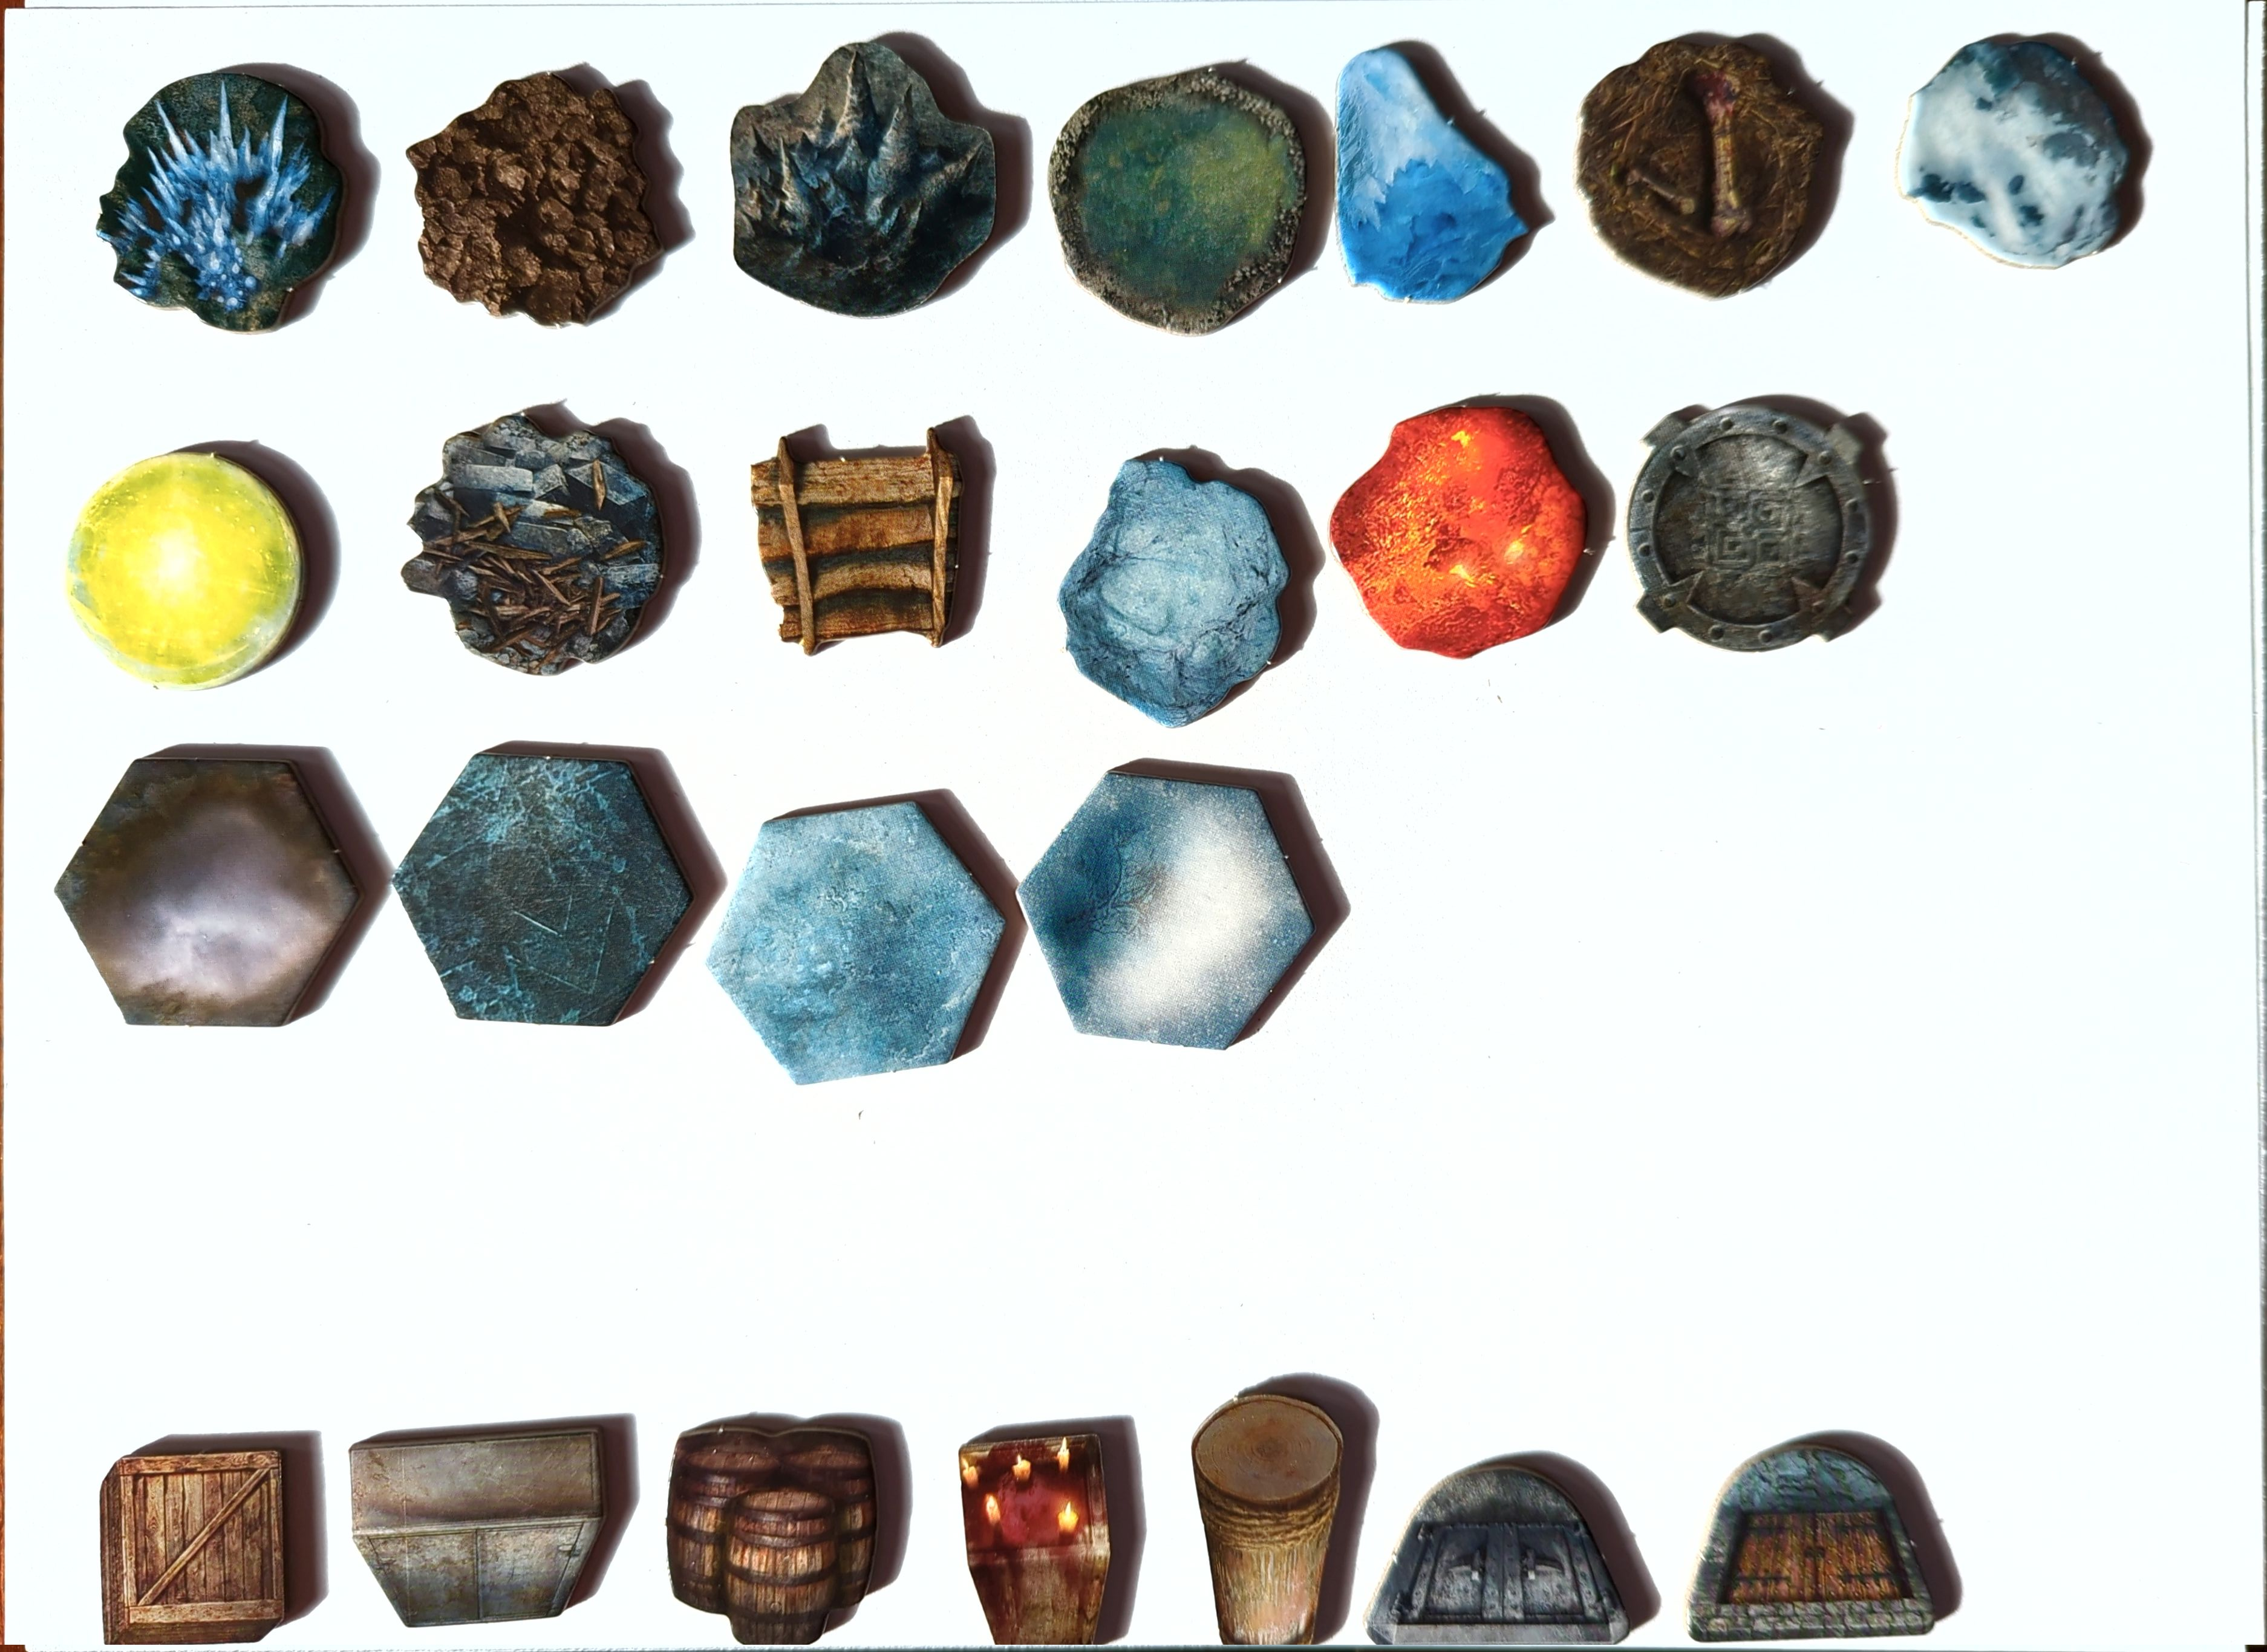
\includegraphics[scale=0.2]{terrain-001.jpg}};
%%%%    \draw[step=1cm,gray] (0,0) grid (26,19);
%%%%    \draw[step=2mm,lightgray,very thin] (0,0) grid (26,19);
%%%%    
%%%%    \foreach \x in {0,1,...,26} {
%%%%      \node[anchor=north] at (\x cm,-0.2 cm) {\x0};
%%%%    }
%%%%    
%%%%    \foreach \x in {0,1,...,26} {
%%%%      \node[anchor=south] at (\x cm,19.2 cm) {\x0};
%%%%    }
%%%%    
%%%%    \foreach \y in {0,1,...,19} {
%%%%      \node[anchor=east] at (-0.1 cm,\y cm) {\y0};
%%%%    }
%%%%    
%%%%    %\begin{scope}
%%%%    %\clip (10cm,153cm) rectangle (45cm,187cm);
%%%%    %\end{scope}
%%%%    \end{tikzpicture}
%%%%    
%%%%    
%%%%    
%%%%    \begin{tikzpicture}[x=1mm,y=1mm]
%%%%    \begin{scope}
%%%%    \clip (10,153) rectangle (45,187);
%%%%    %\clip (0,0) rectangle (10,10);
%%%%    \node[anchor=south west,inner sep=0] (image) at (0,0)
%%%%         {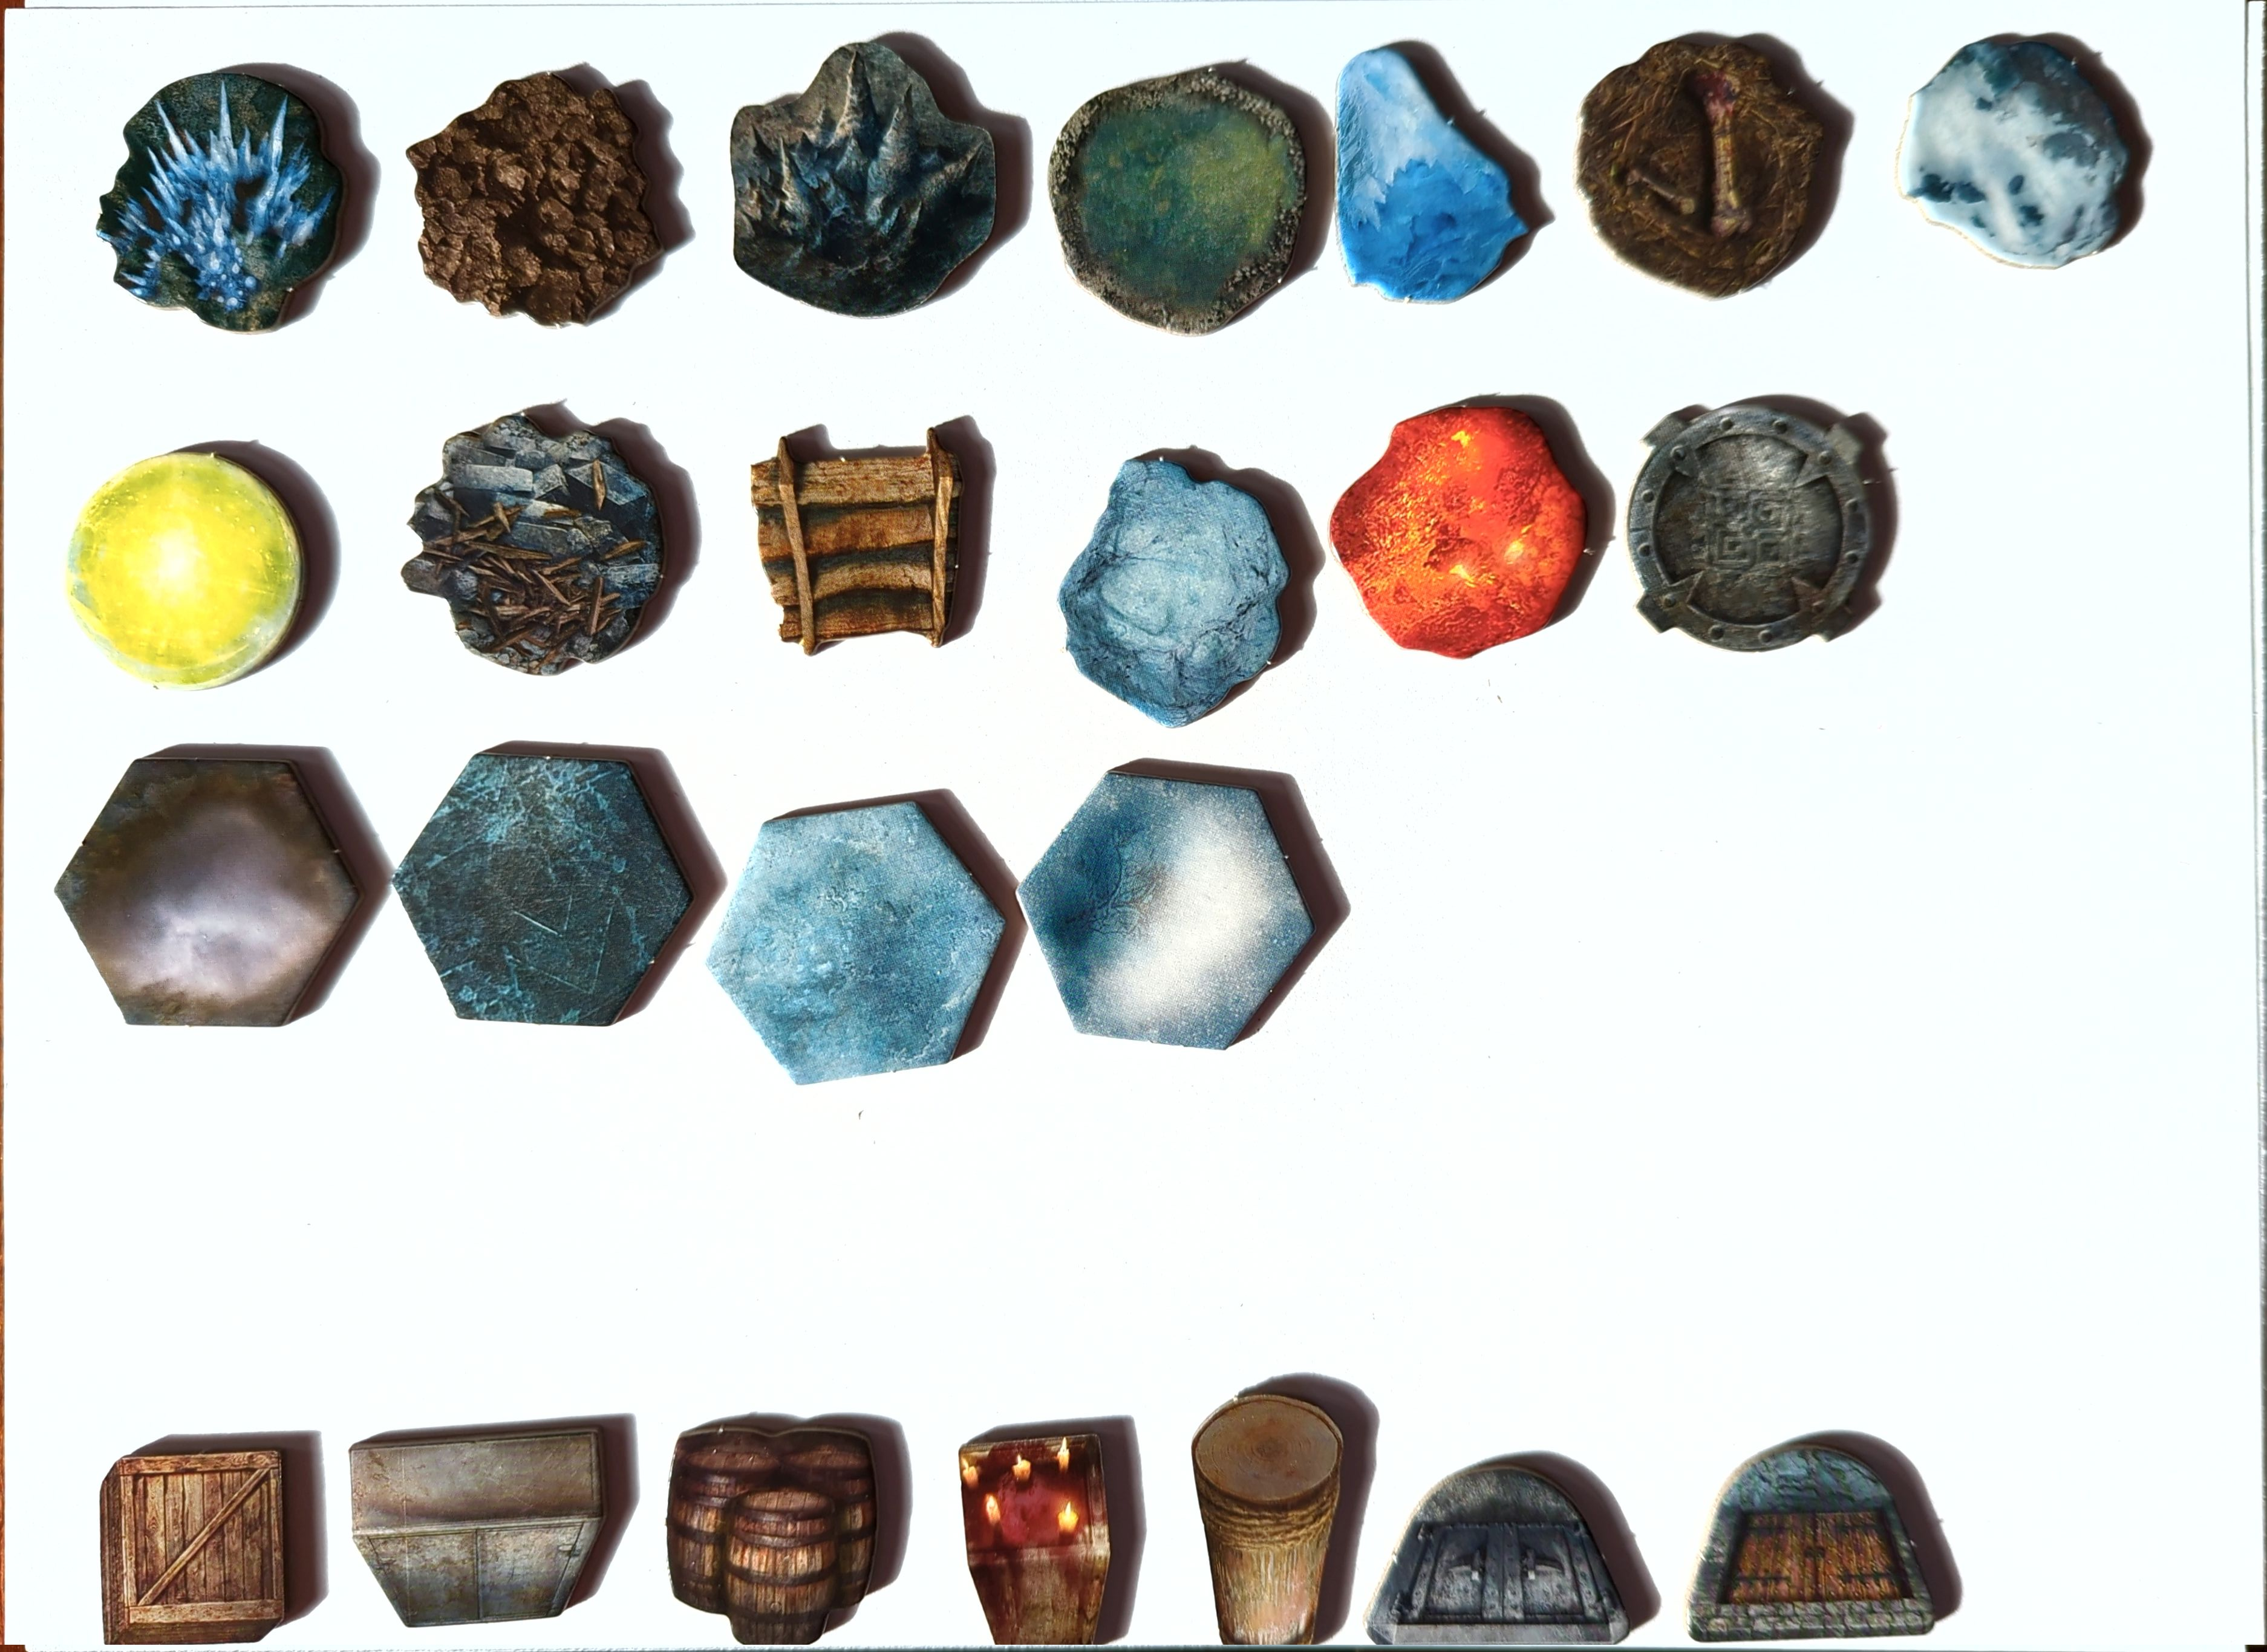
\includegraphics[scale=0.2]{terrain-001.jpg}};
%%%%    \end{scope}
%%%%    
%%%%    \node[below of = image] {Icy Spikes};
%%%%    
%%%%    \draw (image.south west) rectangle (image.north east);
%%%%    \end{tikzpicture}
%%%%    
%%%%    \clearpage

\begin{center}

\begin{tikzpicture}[x=0.2pt,y=0.2pt] % 1 point per pixel

\node[anchor=south west,inner sep=0] (image) at (0,0)
     {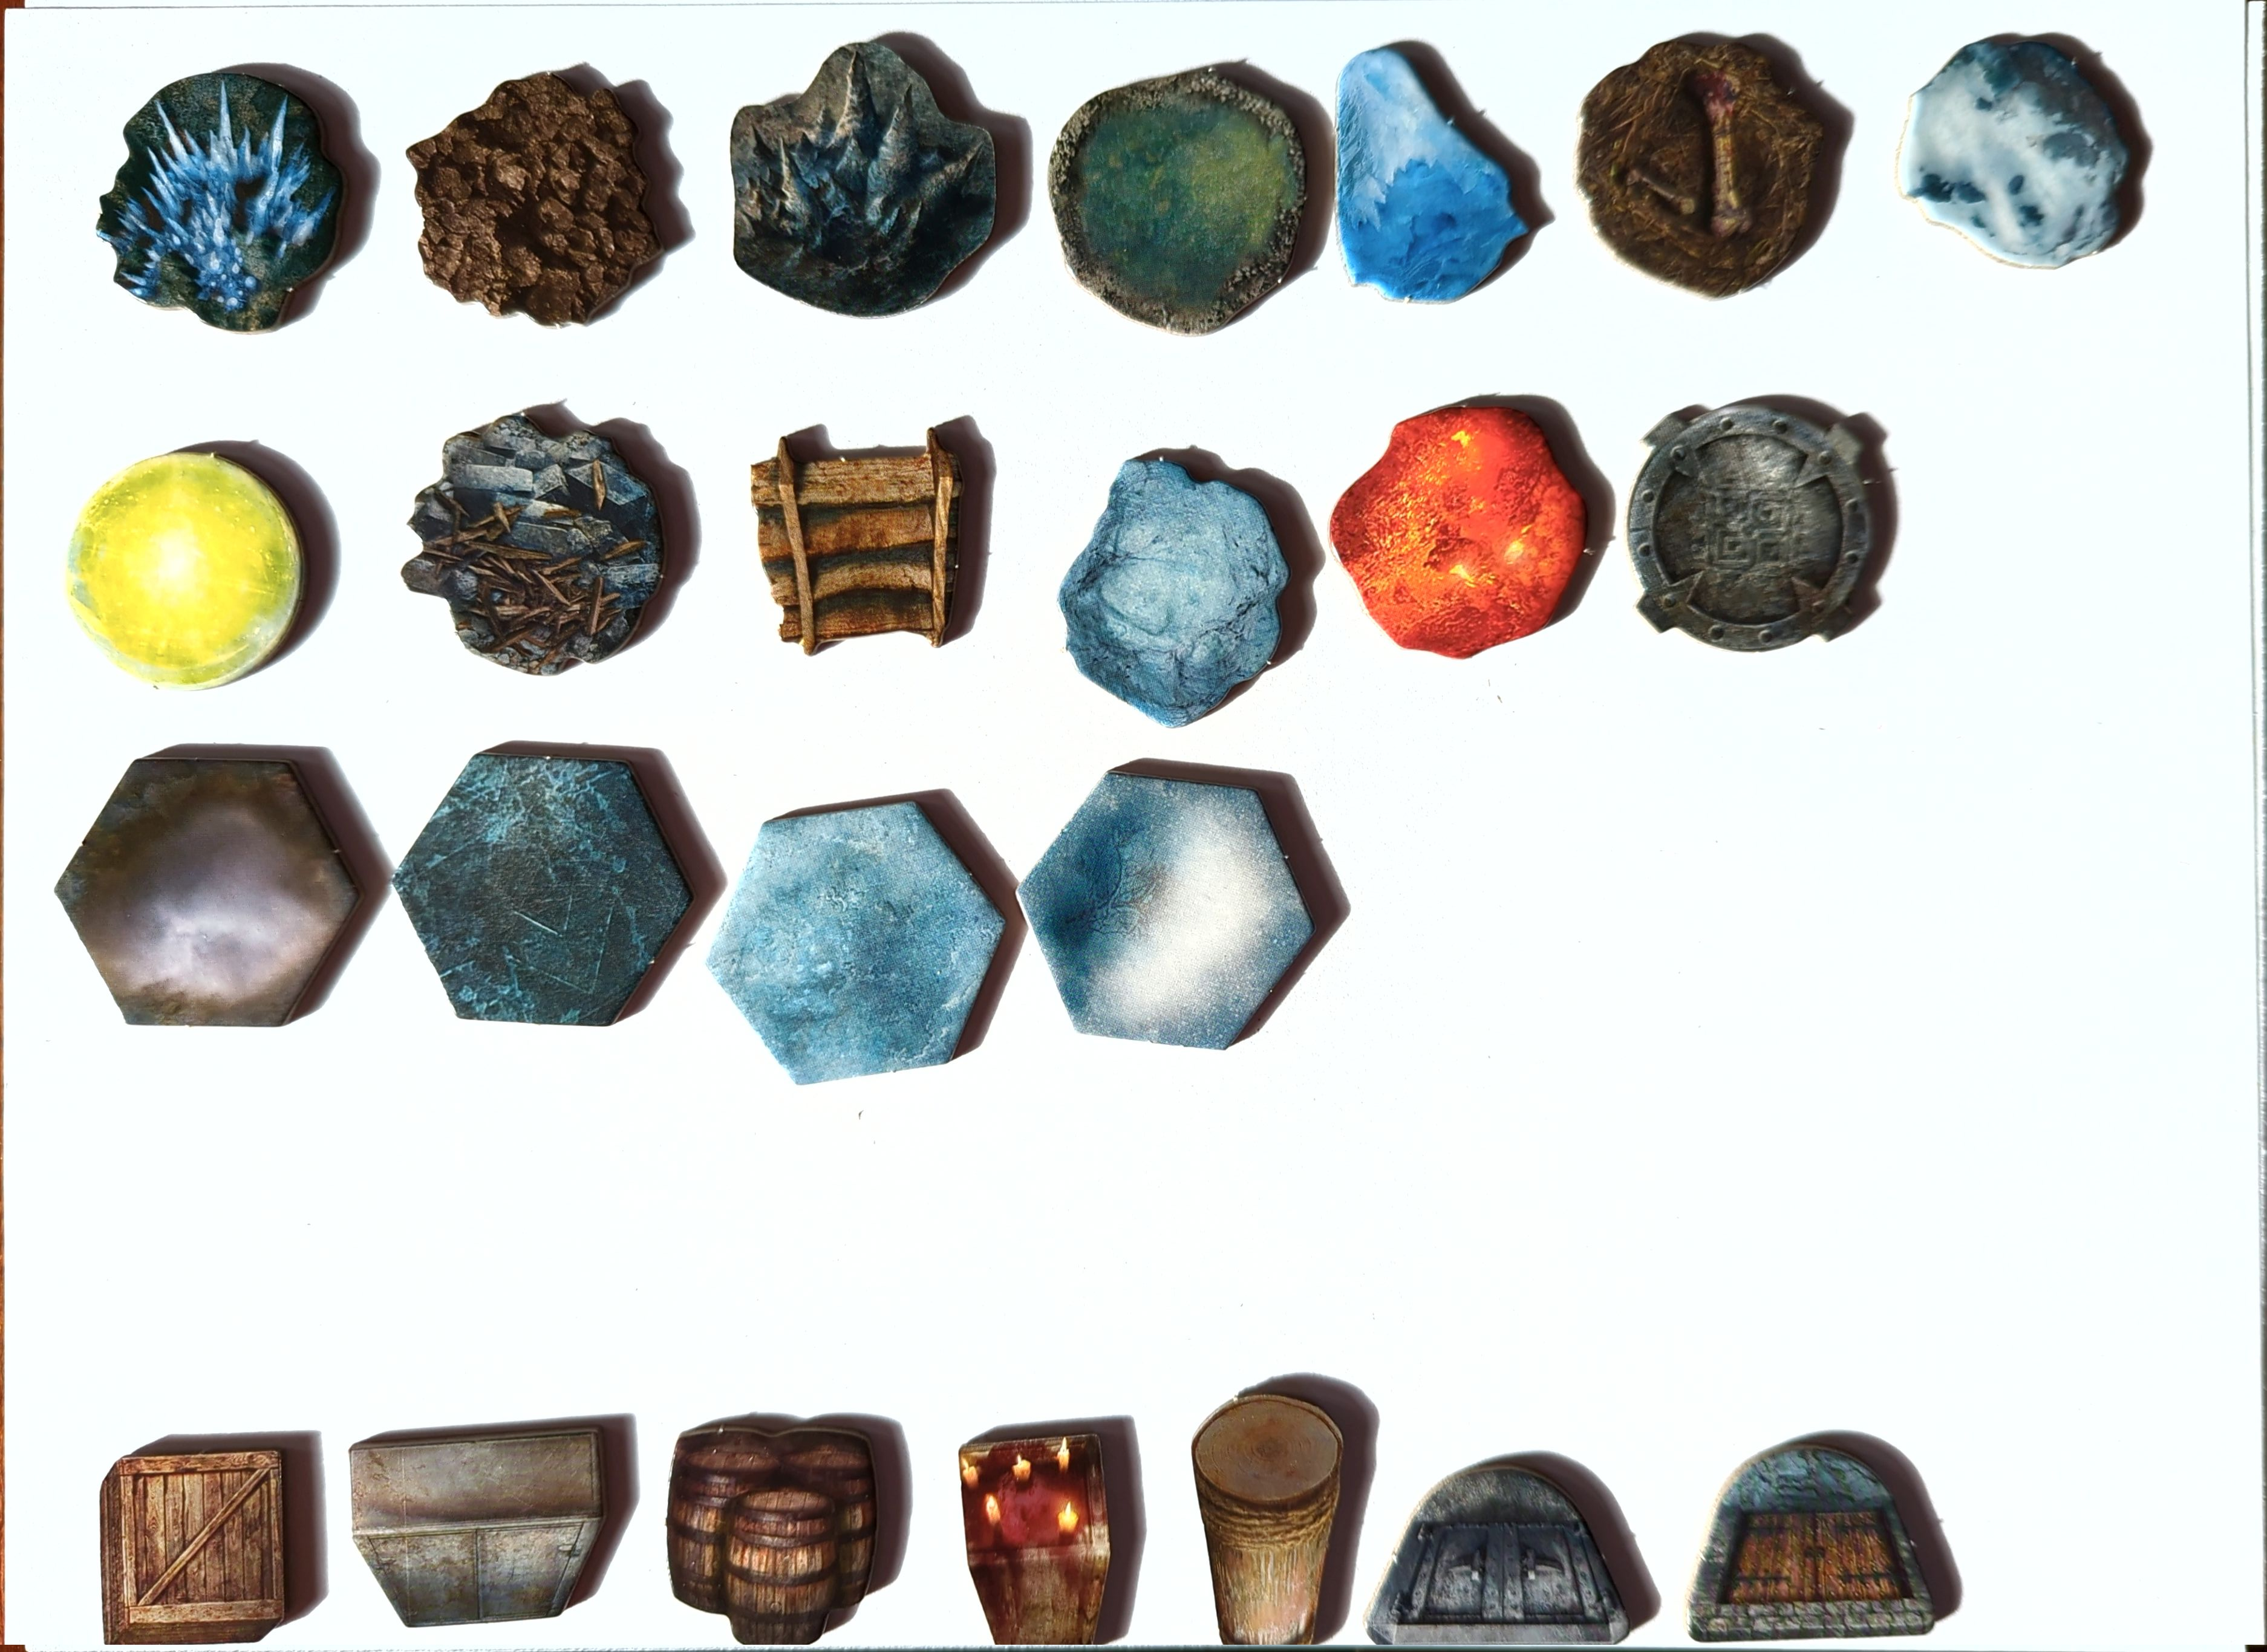
\includegraphics[scale=0.2,viewport=0 0 3748 2732]{terrain-001.jpg}};
\draw[step=100,gray] (0,0) grid (3700,2700);
\draw[step=20,lightgray,very thin] (0,0) grid (3700,2700);
\draw[step=200,darkgray] (0,0) grid (3700,2700);

\foreach \x in {0,200,...,3600} {
  \node[anchor=north] at (\x,-0.2 cm) {\x};
}

\foreach \x in {0,200,...,3600} {
  \node[anchor=center] at (\x,1550) {\x};
}

\foreach \x in {0,200,...,3600} {
  \node[anchor=south] at (\x,2700) {\x};
}

\foreach \y in {0,200,...,2600} {
  \node[anchor=east] at (-0.1 cm,\y) {\y};
}

\end{tikzpicture}

\clearpage

\begin{tikzpicture}[x=0.2pt,y=0.2pt]
\node[anchor=south,inner sep=0] (image) at (0,0)
     {\includegraphics*[scale=0.2,viewport=1230 1640 1660 2100]{terrain-001.jpg}};


\node[anchor=north] (0, -1000) {\LARGE 4 Ladder};
\end{tikzpicture}
\end{center}

\end{document}
